% --------------------------------------------------------------------------- %
% Poster for the ECCS 2011 Conference about Elementary Dynamic Networks.      %
% --------------------------------------------------------------------------- %
% Created with Brian Amberg's LaTeX Poster Template. Please refer for the     %
% attached README.md file for the details how to compile with `pdflatex`.     %
% --------------------------------------------------------------------------- %
% $LastChangedDate:: 2011-09-11 10:57:12 +0200 (V, 11 szept. 2011)          $ %
% $LastChangedRevision:: 128                                                $ %
% $LastChangedBy:: rlegendi                                                 $ %
% $Id:: poster.tex 128 2011-09-11 08:57:12Z rlegendi                        $ %
% --------------------------------------------------------------------------- %
\documentclass[a0paper,portrait]{baposter}

\usepackage{relsize}		% For \smaller
\usepackage{url}			% For \url
% \usepackage{epstopdf}	% Included EPS files automatically converted to PDF to include with pdflatex

%%% Global Settings %%%%%%%%%%%%%%%%%%%%%%%%%%%%%%%%%%%%%%%%%%%%%%%%%%%%%%%%%%%

\graphicspath{{pix/}}	% Root directory of the pictures 
% \tracingstats=2			% Enabled LaTeX logging with conditionals

%%% Color Definitions %%%%%%%%%%%%%%%%%%%%%%%%%%%%%%%%%%%%%%%%%%%%%%%%%%%%%%%%%

\definecolor{bordercol}{RGB}{40,40,40}
\definecolor{headercol1}{RGB}{186,215,230}
\definecolor{headercol2}{RGB}{80,80,80}
\definecolor{headerfontcol}{RGB}{0,0,0}
\definecolor{boxcolor}{RGB}{199,224,236}
%\definecolor{boxcolor}{RGB}{195,217,255}
%\definecolor{boxcolor}{RGB}{251,255,185}

%%%%%%%%%%%%%%%%%%%%%%%%%%%%%%%%%%%%%%%%%%%%%%%%%%%%%%%%%%%%%%%%%%%%%%%%%%%%%%%%
%%% Utility functions %%%%%%%%%%%%%%%%%%%%%%%%%%%%%%%%%%%%%%%%%%%%%%%%%%%%%%%%%%

%%% Save space in lists. Use this after the opening of the list %%%%%%%%%%%%%%%%
\newcommand{\compresslist}{
	\setlength{\itemsep}{1pt}
	\setlength{\parskip}{0pt}
	\setlength{\parsep}{0pt}
}

%%%%%%%%%%%%%%%%%%%%%%%%%%%%%%%%%%%%%%%%%%%%%%%%%%%%%%%%%%%%%%%%%%%%%%%%%%%%%%%
%%% Document Start %%%%%%%%%%%%%%%%%%%%%%%%%%%%%%%%%%%%%%%%%%%%%%%%%%%%%%%%%%%%
%%%%%%%%%%%%%%%%%%%%%%%%%%%%%%%%%%%%%%%%%%%%%%%%%%%%%%%%%%%%%%%%%%%%%%%%%%%%%%%

\begin{document}
\typeout{Poster rendering started}

%%% Setting Background Image %%%%%%%%%%%%%%%%%%%%%%%%%%%%%%%%%%%%%%%%%%%%%%%%%%
\background{
	\begin{tikzpicture}[remember picture,overlay]%
	\draw (current page.north west)+(-2em,2em) node[anchor=north west]
	{
\includegraphics[height=1.1\textheight]{background}};
	\end{tikzpicture}
}

%%% General Poster Settings %%%%%%%%%%%%%%%%%%%%%%%%%%%%%%%%%%%%%%%%%%%%%%%%%%%
%%%%%% Eye Catcher, Title, Authors and University Images %%%%%%%%%%%%%%%%%%%%%%
\begin{poster}{
	grid=false,
	% Option is left on true though the eyecatcher is not used. The reason is
	% that we have a bit nicer looking title and author formatting in the headercol
	% this way
	%eyecatcher=false, 
	borderColor=bordercol,
	headerColorOne=headercol1,
	headerColorTwo=headercol2,
	headerFontColor=headerfontcol,
	% Only simple background color used, no shading, so boxColorTwo isn't necessary
	boxColorOne=boxcolor,
	headershape=roundedright,
	headerfont=\Large\sf\bf,
	textborder=rectangle,
	background=user,
	headerborder=open,
  boxshade=plain
}
%%% Eye Cacther %%%%%%%%%%%%%%%%%%%%%%%%%%%%%%%%%%%%%%%%%%%%%%%%%%%%%%%%%%%%%%%
{
	Eye Catcher, empty if option eyecatcher=false - unused
}
%%% Title %%%%%%%%%%%%%%%%%%%%%%%%%%%%%%%%%%%%%%%%%%%%%%%%%%%%%%%%%%%%%%%%%%%%%
{\sf\bf
	Active Learning based \\ 
    MCMC-free Bayesian inversion
}
%%% Authors %%%%%%%%%%%%%%%%%%%%%%%%%%%%%%%%%%%%%%%%%%%%%%%%%%%%%%%%%%%%%%%%%%%
{
	\vspace{1em} \underline{R. Ancarola}, B. Sudret$^1$, S. Marelli$^1$,M. Picasso$^2$\\
    $\prescript{1}{}{\text{ETH: {\smaller Chair of Risk, Safety and Uncertainty Quantification}}}$,
	$\prescript{2}{}{\text{EPFL}}$
}
%%% Logo %%%%%%%%%%%%%%%%%%%%%%%%%%%%%%%%%%%%%%%%%%%%%%%%%%%%%%%%%%%%%%%%%%%%%%
{
% The logos are compressed a bit into a simple box to make them smaller on the result
% (Wasn't able to find any bigger of them.)
\setlength\fboxsep{0pt}
\setlength\fboxrule{0.5pt}
	%\fbox{
		\begin{minipage}{14em}
			
\includegraphics[width=10em,height=4em]{logo.png}
			%
\includegraphics[width=4em,height=4em]{eth-logo} \\
			\\

            %\hspace*{-1.5in}
            
\includegraphics[width=10em,height=2.7em]{eth_logo}
			%
\includegraphics[width=4em,height=4em]{aitia_logo}
		\end{minipage}
	%}
}

\headerbox{Abstract}{name=abstract,column=0,row=0}{

%The computation of likelihood function evaluation can take minutes or even hours, it's then fundamental to limit the number of likelihood calls.
%Active Learning Reliability (ARL) \cite{arl, bbus} is a framework exploiting surrogate model techniques and uncertainty quantification which allows to gain information around the limit state surface while limiting at the same time the number of forward model evaluations.
In this master thesis we explore and extend a recently proposed method to perform \textit{Bayesian inversion}, focusing on the reconstruction of the \textit{likelihood function} by combining \textit{active learning} \cite{arl} and \textit{Polynomial chaos Kriging} (PCK) \cite{pck}.
The basic idea is exploiting the recently proposed framework of \textit{Bayesian Updating with Structural Reliability} (BUS) \cite{bus}, which allows one to express the general \textit{Bayesian inference} formulation into a \textit{Structural Reliability} (SR) problem and rare event estimation.
\par\noindent
The \textit{active learning} approach allows to fix a limited budget to the \textit{forward model} evaluations for the PCK reconstruction, thus furnishing a cheap evaluator of the likelihood function in the most important regions.
%More specifically, a Polynomial Chaos Kriging (PCK) \cite{pck}  surrogate is adopted for the log-likelihood function and SuS is used to computationally solve the Bayesian inverse problem. 
}

\headerbox{Bayesian inversion}{name=problem,column=0,row=0,below=abstract}{
%In a context of Uncertainty Quantification, the assessment of  physical computational models response 
%\par\noindent
Bayesian inversion exploits Bayes theorem to infer the probability distribution $\pi$ associated to a random variable $\vec{X} \in \Dx \subset \R^M$. 

%$\vec{X} \in \Dx$ basing on real observed data $\mathcal{Y} \in \Dy$. The likelihood $\Lk : \Dx \rightarrow \R$ expresses the probability density function of observations inferred by given parameters and 

\begin{itemize}
\item $\pi : \Dx \rightarrow \R$, prior distribution.
\item $\Lk : \Dx \rightarrow \R$, likelihood distribution expressing evidence of \\
observations $\vec{y} \in \mathcal{D}_{\vec{Y}} \subset \R^N$ affecting $\vec{X}$.
\end{itemize}

{\smaller
$$
\pi(\vec{x}|\vec{y}) = \frac{\Lk(\vec{x};\vec{y}) \pi(\vec{x})}{\mathcal{Z}}, \quad \mathcal{Z} \stackrel{\text{def}}{=} \int\limits_{\Dx} \Lk(\vec{x};\vec{y}) \pi(\vec{x}) d\vec{x}
$$
}

is called the distribution of $\vec{X}$ posterior to the observations $\vec{y}$. 
}

\headerbox{Subset simulation}{name=suspck,column=0,row=0,below=problem}{
Subset Simulation (SuS) \cite{sus} is suitable for the estimation of the probability of rare events, such as the failure probability in a SR framework. 
%allowing to computationally solve the Bayesian inverse problem.

\par\noindent
\\
The failure domain $F$ and it's associated probability $\mathbb{P}(F)$ are determined by a stochastic search procedure involving $r+1$ subsets of $\Dx$:

\begin{itemize}
\item {\smaller
$ F = F_{r+1} \subset F_r \subset F_{r-1} \subset \dots \subset F_1 \subset  F_0 = \Dx$
}
\item {\smaller $\mathbb{P}(F) = \prod\limits_{i=1}^{r+1} \mathbb{P}(F_i|F_{i-1}) =: \left( \frac{1}{10}\right)^r \mathbb{P}(F_{r+1}|F_r)$
}
\end{itemize}

%\par\noindent
%A limit state function is 
%Samples belonging to $F_r$ are determined such that at least $10\%$ of them are also BuS posterior samples, as they lie on the BuS failure domain $F$. Their distribution is a truncation of the prior:
Samples from each subset are generated by a MCMC routine which targets the distribution:
{\small$$ \pi(p, \vec{x}|F_i) \propto \mathbbm{1}_{F_i}(p, \vec{x}) \pi(\vec{x}), \quad 
i = 0,\dots,r+1$$}

The algorithm stops ($i = r$) when $h(p, \vec{x}) \le 0$ for at least $10\%$ of the samples.
$\mathbb{P}(F_{r+1}|F_r)$ is Monte Carlo estimated with $F_r$ samples.
}


\headerbox{References}{name=references,column=0,below=suspck,above=bottom}{
\smaller													% Make the whole text smaller
\vspace{-0.4em} 										% Save some space at the beginning
\bibliographystyle{plain}							% Use plain style
\renewcommand{\section}[2]{\vskip 0.05em}		% Omit "References" title
{\footnotesize
\begin{thebibliography}{1}							% Simple bibliography with widest label of 1
\itemsep=-0.01em										% Save space between the separation
\setlength{\baselineskip}{0.4em}					% Save space with longer lines
%\bibitem{bayesinv} Tarantola, Albert: \emph{Inverse Problem Theory and Methods for Model Parameter Estimation}
\bibitem{bus} Daniel Straub  and Iason Papaioannou: \emph{Bayesian Updating with Structural Reliability Methods}
\bibitem{sus} Siu-Kui Au and James L. Beck: \emph{Estimation of small failure probabilities in high dimensions by subset simulation}.
\bibitem{arl} Rui Teixeira and Maria Nogal and Alan O'Connor: \emph{Adaptive approaches in metamodel-based reliability analysis: A review}.
%\bibitem{bbus} D. Rossat and J. Baroth and M. Briffaut and F. Dufour : \emph{Bayesian inversion using adaptive Polynomial Chaos Kriging within Subset Simulation}.
\bibitem{pck} Pierric Kersaudy and Bruno Sudret and Nadège Varsier and Odile Picon and Joe Wiart : \emph{A new surrogate modeling technique combining Kriging and polynomial chaos expansions - Application to uncertainty analysis in computational dosimetry}
\end{thebibliography}
}

}

% Column end

\headerbox{BuS framework and posterior sampling}{name=bus,span=2,column=1,row=0}{
%\headerbox{BuS framework}{name=bus,column=0,row=0,below=problem}{
%Introduced by \cite{bus}, the Bayesian update Structural Reliability (BuS) framework casts Bayesian inversion into an equivalent Structural Reliability (SR) problem.
%\par\noindent
By considering $P \sim \mathcal{U}(0,1)$ and the joint random variables $(P, \vec{X})$, one defines the limit state function $h : [0,1] \times \Dx \rightarrow \R$ which usually corresponds in SR to the difference between a resistance (R) contribution and a stress (S) contribution.
{\smaller
$$
h(p, \vec{x}) = R(p) - S(\vec{x}) = p - c \Lk(\vec{x};\vec{y}), \quad
c > 0
$$
}
%In SR, the failure domain $F$ it's characterized by $h(p, \vec{x}) \le 0$ and the failure probability $\mathbb{P}_f$ is the probability associated to $F$.
%\par\noindent
BuS rewrites the posterior distribution in terms of a marginal probability over the failure domain $F$
{\smaller
$$
\pi(\vec{x}|\vec{y}) = \frac{\pi(\vec{x})}{c\mathcal{Z}} \int_0^{c\Lk(\vec{x};\vec{y})}  dp = \frac{1}{\mathbb{P}(F)} \int_0^1 \mathbbm{1}_F(p, \vec{x}) \pi(\vec{x}) dp, \quad
F \stackrel{\text{def}}{=} \{(p,\vec{x}) : h(p, \vec{x}) \le 0\}
$$
}

%Subset Simulation (SuS) \cite{sus} is suitable for the efficient estimation of small probabilities, such as the failure probability of SR problems. 
Subset Simulation is adopted for the sampling procedure of posterior $(P, \vec{X})$:
{\smaller
$$
\pi(p,\vec{x}|F) = \pi(p,\vec{x}|F_{r+1}) \propto \mathbbm{1}_{F_{r+1}}(p,\vec{x}) \pi(\vec{x})
$$
}
\begin{center}
\begin{minipage}{0.85\textwidth}
\centering
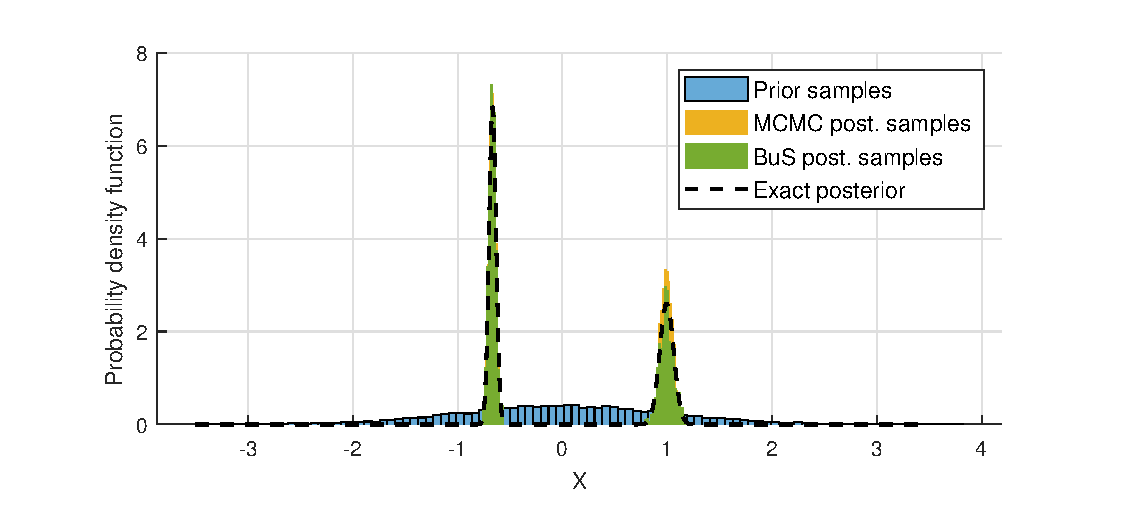
\includegraphics[width=0.75\textwidth]{post_apocalyptic.eps}
\captionof*{figure}{BuS-SuS posterior distribution compared to the exact posterior distribution and a classical MCMC approach sampling for a specific two-peaked test case of Bayesian inversion.}
\end{minipage}
\end{center}
}

\headerbox{Likelihood Active Learning}{name=lal,span=2,column=1,row=0, below=bus,above=bottom}{

%The Bayesian inverse problem rewritten into BuS framework can be solved exploiting Subset Simulation (SuS) \cite{}, which is suitable for the estimation of the probability of rare events, such as the failure probability $\mathbb{P}_f$. %By setting $c^{-1} = \max_{\vec{x} \in \Dx} \Lk(\vec{x})$, the failure probability $\mathbb{P}_f$ can be extremely small
%In real applications, the computation of likelihood function evaluation can take minutes or even hours, it's then fundamental to limit the number of likelihood calls.
%Active Learning Reliability (ARL) \cite{arl, bbus} is a framework exploiting surrogate model techniques and uncertainty quantification which allows to gain information around the limit state surface (in BuS, $h(p, \vec{x}) \approx 0$) while limiting at the same time the number of forward model evaluations.
%More specifically, a Polynomial Chaos Kriging (PCK) \cite{pck}  surrogate is adopted for the log-likelihood function and SuS is used to computationally solve the Bayesian inverse problem. 

\begin{multicols}{2}

\par\noindent
Starting from a set of initial training points, also called \textit{Experimental Design} (ED):
\begin{itemize}
\item $\mathcal{X} = \{\vec{x}^{(1)}, \dots, \vec{x}^{(N_0)}\} \subset \Dx$ 
\item $L = \{\Lk(\vec{x}^{(1)}), \dots, \Lk(\vec{x}^{(N_0)})\} \subset \R$
\end{itemize}
Likelihood Active Learning enriches $\mathcal{X}$ and $L$ in high probability zones. 

\par\noindent
The basic iterative procedure is composed of the following steps: 

\begin{enumerate}
\item Construct surrogate PCK $\hat{\ell}$ of $\log(\Lk)$ using current $\mathcal{X}$ and $L$.
\item Retrieve samples $\{(p_k,\vec{x}_k)\}_{k=1}^K$ distributed according to the subset $F_r$ of SuS using the surrogate limit state function
{\small $$ h_\ell(p,\vec{x}) = \log(p) - \log(c) - \hat{\ell}(\vec{x})$$}
\item Evaluate learning function and find best candidate for enrichment:
{\small $$\vec{x}^* = \argmin\limits_{k = 1,\dots,K} \frac{|\E[h_\ell(p_k, \vec{x}_k)]|}{\sqrt{\text{var}[h_\ell(p_k, \vec{x}_k)]}}$$}
\item Append $\vec{x}^*$ to $\mathcal{X}$ and $\Lk(\vec{x}^*)$ to $L$ and repeat from 1. until the target size ($> N_0$) is reached.
\end{enumerate} 

\columnbreak

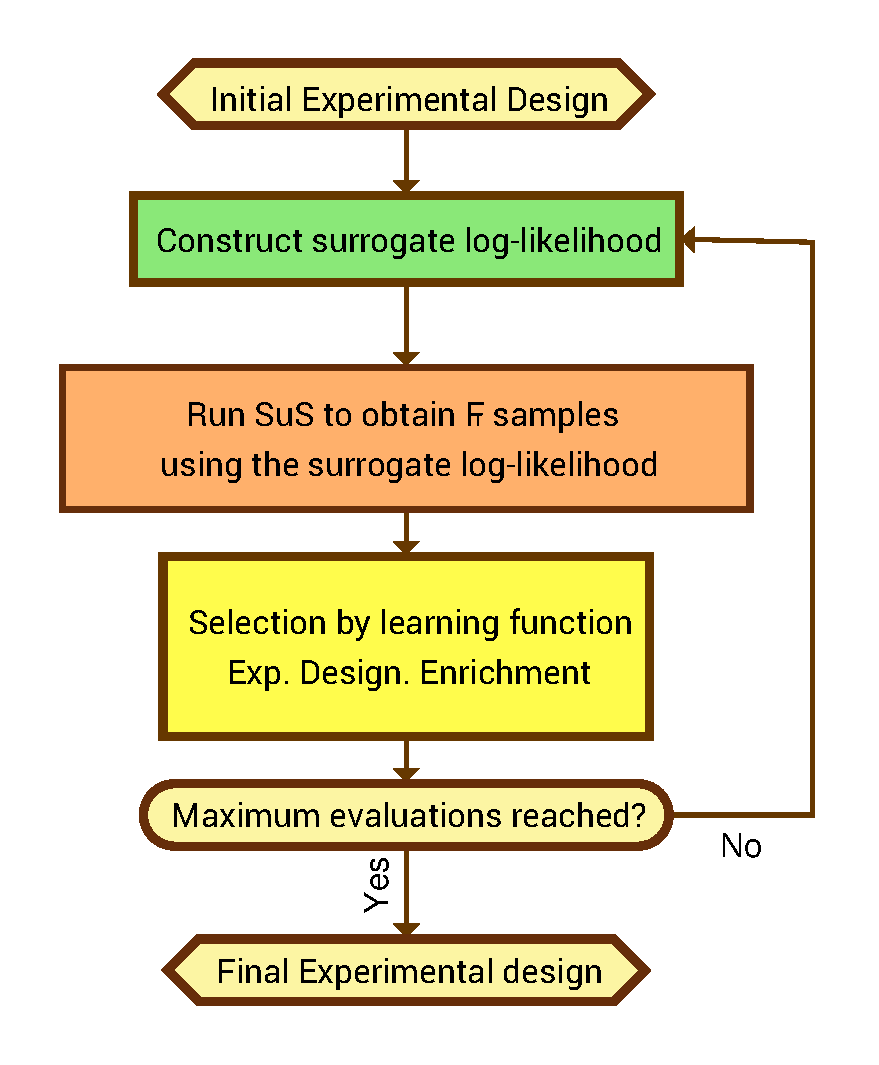
\includegraphics[width=0.5\textwidth]{schema_transparent.pdf}
\end{multicols}

\begin{minipage}{\textwidth}
    \centering
    \begin{minipage}{0.48\textwidth}
    \centering
        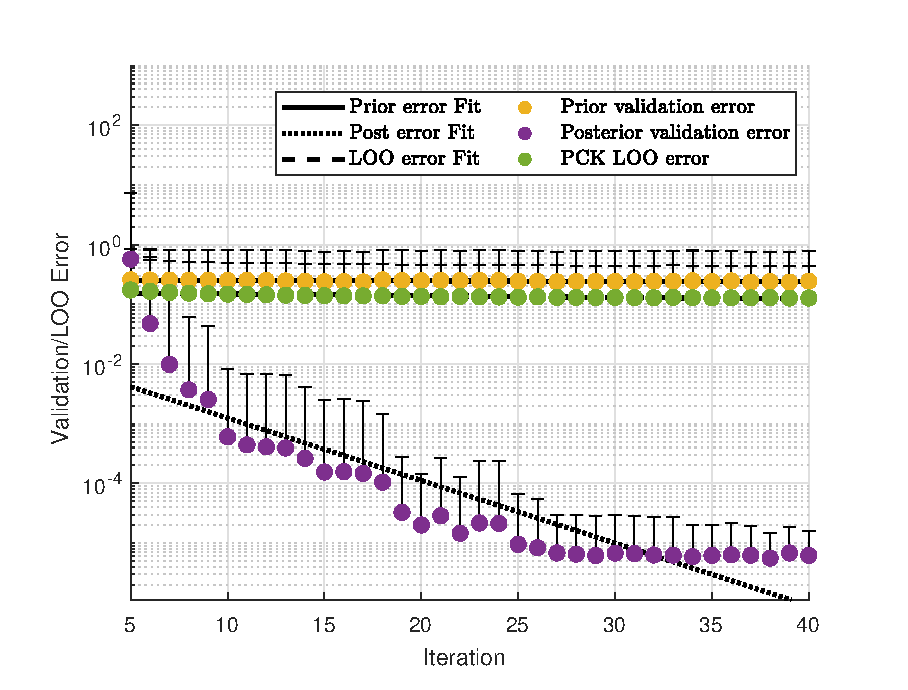
\includegraphics[width=0.9\textwidth]{validation_stat.eps}
        \captionof*{figure}{Validation error for the two-peaked test case along Likelihood Active Learning iterations.}
        %for the two-peaked Gaussian mixture case.}
    \end{minipage}
    \hspace{0.1cm}
    \begin{minipage}{0.48\textwidth}
        \centering
        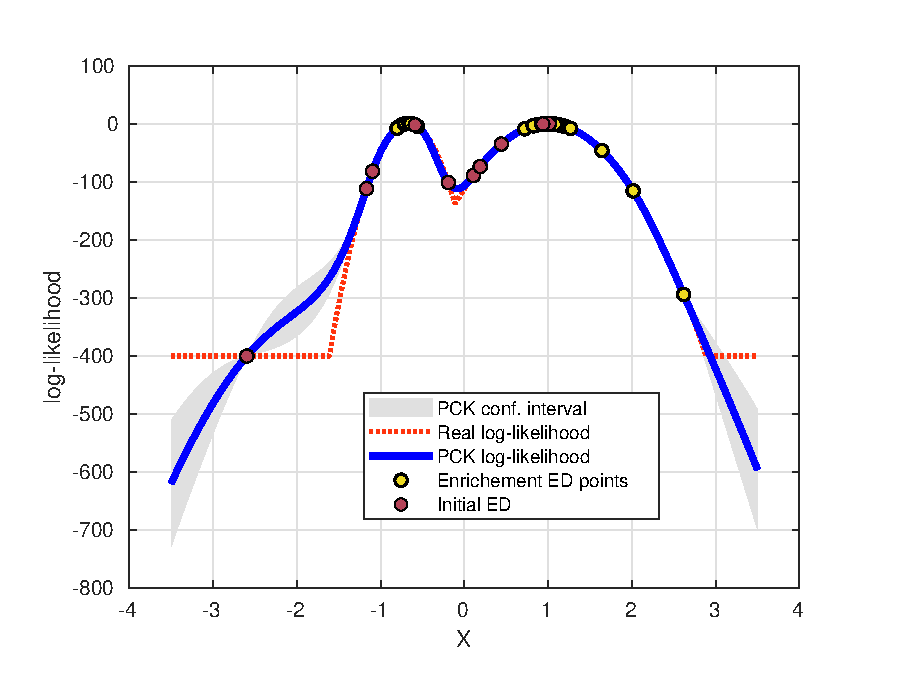
\includegraphics[width=0.9\textwidth]{kriging.eps}
        \captionof*{figure}{PCK visualization of Likelihood Active Learning enrichment for a two-peaked likelihood test case.}
    \end{minipage}
\end{minipage}

}



\end{poster}
\end{document}
